% !TeX root = ../main.tex
\section{Proposed System Architecture}
\label{sec:arquitectura}

To provide federated learning with robust traceability and Byzantine fault resilience, we propose a hybrid architecture decoupled into three operational planes~\cite{zhao2021privacy, trautwein2022design}: the federated computation plane (Flower), the off-chain content-addressable storage plane (IPFS), and the on-chain consensus and immutability plane (Hyperledger Besu). Figure~\ref{fig:arq_sistema} illustrates the end-to-end interaction among these components.

\begin{figure}[htbp]
    \centering
    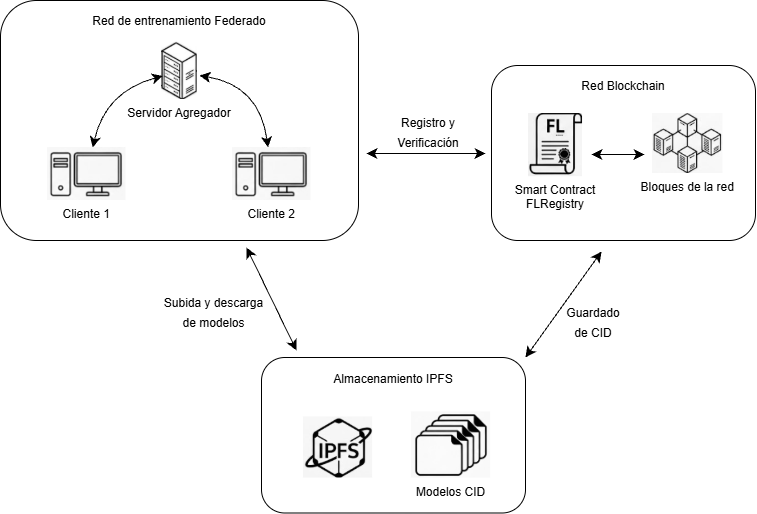
\includegraphics[width=0.88\textwidth]{figures/ArqSistema.png}
    \caption{Overall hybrid system architecture: decoupling between federated computation (Flower), off-chain parameter storage (IPFS), and immutable traceability logging (Hyperledger Besu with IBFT 2.0).}
    \label{fig:arq_sistema}
\end{figure}

\subsection{Smart Contract Design: FLRegistry}
Governance and audit logic are encapsulated within the \texttt{FLRegistry} smart contract, implemented in Solidity (compiler version \texttt{0.8.10}). Its primary objective is to maintain a deterministic, chronological audit log of each federated round without storing massive numerical parameter matrices on-chain.

\subsubsection{Data Structures and Persistence}
The core entity within the contract is the \texttt{ModelRound} structure, defined as:
\begin{verbatim}
struct ModelRound {
    uint256 roundNum;
    string modelHash;
    address author;
    uint256 timestamp;
}
\end{verbatim}
where \texttt{roundNum} indexes the federated iteration, \texttt{modelHash} stores the IPFS Content Identifier (CIDv0, encapsulating the SHA-256 multihash of the serialized model), \texttt{author} records the Ethereum public address of the sender (\texttt{msg.sender}), and \texttt{timestamp} captures the block validation timestamp.

Contract state is organized through two complementary mappings:
\begin{itemize}
    \item \texttt{mapping(uint256 => ModelRound) public history}: sequentially records the global models aggregated by the coordinator at the conclusion of each round $t$.
    \item \texttt{mapping(uint256 => mapping(address => ModelRound)) public clientHistory}: indexes the individual local contributions submitted by each client in each round, enabling granular forensic auditing.
\end{itemize}

Additionally, state pointers \texttt{latestRound} and boolean flag \texttt{hasModel} are maintained to facilitate direct and constant-time read access without requiring iterative storage scans.

\subsubsection{State-Modifying Primitives and Access Control}
The contract exposes two state-modifying transactional functions that emit the decoupled \texttt{ModelUpdated} event:
\begin{itemize}
    \item \texttt{registerClientModel(uint256 round, string memory hash)}: Invoked by each edge client $k$ upon completing local training, immutably binding the CID of its contribution to its Ethereum address (\texttt{msg.sender}).
    \item \texttt{updateModel(uint256 round, string memory hash)}: Invoked operationally by the aggregation coordinator after executing the aggregation algorithm. To enforce consortium governance and prevent unauthorized participants or rogue nodes from submitting fraudulent global models, this function is guarded by the \texttt{onlyServer} access control modifier:
    \begin{verbatim}
modifier onlyServer() {
    require(msg.sender == serverAddress, 
            "Unauthorized sender");
    _;
}
    \end{verbatim}
    where \texttt{serverAddress} is initialized in the contract constructor with the authorized coordinator public address (which can be reassigned or governed via consortium multi-signature schemes). Consequently, the EVM deterministically reverts any unauthorized call to \texttt{updateModel}.
\end{itemize}

\subsubsection{Read and Verification Primitives}
To avoid imposing execution costs during routine checks, model verification queries are implemented as \texttt{view} functions, resolved locally at the JSON-RPC node without consuming gas:
\begin{itemize}
    \item \texttt{getLastModel()}: Enables any client to retrieve the CID of the latest consolidated global model along with its validation timestamp.
    \item \texttt{getClientModel(uint256 round, address client)}: Enables the coordinator and external auditors to cross-check the CID reported by a client against its signed on-chain record.
\end{itemize}

\subsubsection{Model-Agnostic Design and Generalization}
The proposed framework is architecturally and operationally agnostic to neural network topology, data modality, and training framework. Because \texttt{FLRegistry} processes exclusively uniform 46-character string identifiers (the IPFS CIDs encapsulating the multihash digest of the serialized weights), EVM gas costs remain predictable and entirely decoupled from model parameter dimensions—whether the weights represent a shallow classifier, a deep convolutional network, or a Transformer architecture. Similarly, the IPFS storage plane treats serialized parameters as generic byte payloads, making this bidirectional verification protocol directly applicable across diverse modalities (tabular data, time series, acoustic signals, or computer vision) and federated optimization algorithms.

\subsection{Operational Workflow and Bidirectional Cross-Verification}
The federated lifecycle consists of a one-time bootstrap phase followed by an iterative protocol featuring strict bidirectional verification, detailed below:

\subsubsection{Phase 0: Bootstrap and Baseline Model (Round 0)}
Prior to concurrent training execution:
\begin{enumerate}
    \item The Hyperledger Besu network operating under IBFT 2.0 consensus and the IPFS daemon are initialized.
    \item \texttt{FLRegistry} is deployed, and its contract address and ABI are published in a shared configuration manifest.
    \item The coordinator instantiates the initial model parameters $w^{(0)}$, serializes them, and uploads them to IPFS, obtaining the initial identifier $\text{CID}_0$.
    \item The coordinator executes \texttt{updateModel(0, }$\text{CID}_0$\texttt{)}, establishing an auditable cryptographic baseline for all participants.
\end{enumerate}

\subsubsection{Phase 1: Downward Verification (Client Verifies Server)}
Upon receiving the round start signal and candidate weights $w_{cand}^{(t)}$ via gRPC (Figure~\ref{fig:flujo_cliente_verif}):
\begin{enumerate}
    \item The client queries the blockchain by calling \texttt{getLastModel()}, retrieving the officially committed $\text{CID}_{reg}^{(t-1)}$.
    \item The client fetches the referenced model artifact from IPFS and performs an exhaustive, element-wise numerical comparison across all tensor layers against $w_{cand}^{(t)}$ (verifying parametric equality within a floating-point tolerance of $\epsilon = 10^{-7}$).
    \item If any discrepancy is detected between the delivered weights and the on-chain commitment, the client \textbf{aborts training immediately}, effectively neutralizing split-view attacks where a compromised coordinator attempts to distribute biased models selectively to specific clients.
\end{enumerate}

\begin{figure}[htbp]
    \centering
    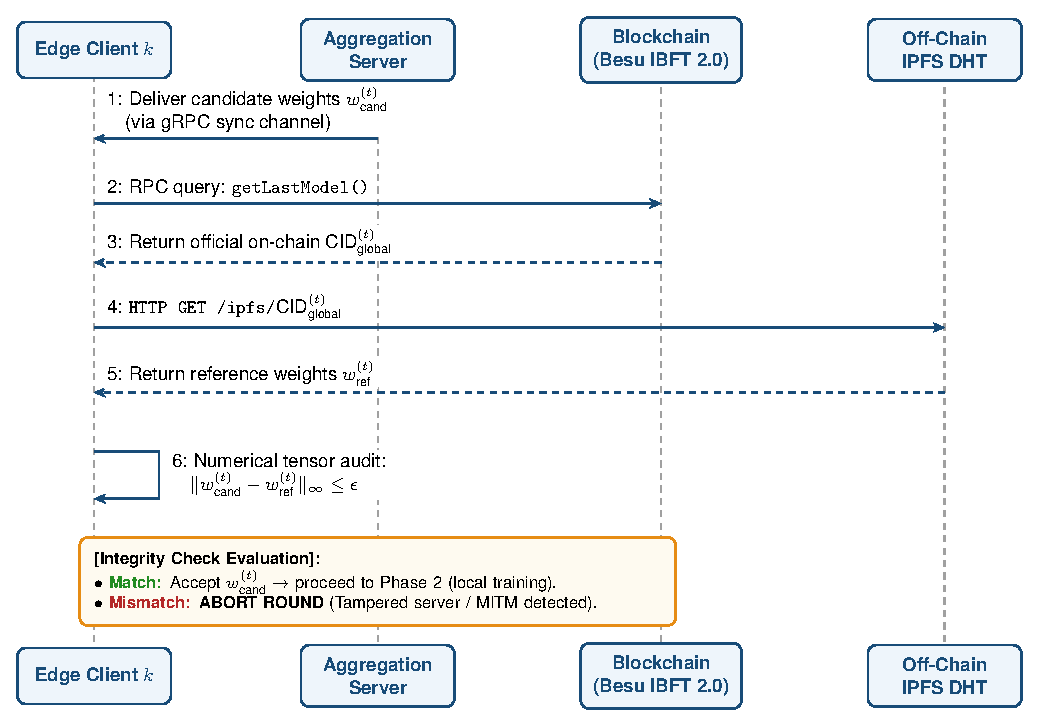
\includegraphics[width=\columnwidth]{figures/flujo_fase1_verificacion_descendente.pdf}
    \caption{Phase 1: Downward verification at the edge client: validating received candidate weights against the on-chain registered CID retrieved from IPFS.}
    \label{fig:flujo_cliente_verif}
\end{figure}

\subsubsection{Phase 2: Local Training and Contribution Commitment}
If the downward verification check passes successfully (Figure~\ref{fig:flujo_cliente_entreno}):
\begin{enumerate}
    \item The client performs local training on its private data partition.
    \item It serializes the updated local weight vector $w_k^{(t)}$ and uploads it to IPFS, obtaining $\text{CID}_k^{(t)}$.
    \item It broadcasts a signed transaction calling \texttt{registerClientModel(}$t$, $\text{CID}_k^{(t)}$\texttt{)} and awaits confirmation within an IBFT 2.0 block receipt.
    \item It returns the parameter payload along with $\text{CID}_k^{(t)}$ and its public key to the Flower coordinator.
\end{enumerate}

\begin{figure}[htbp]
    \centering
    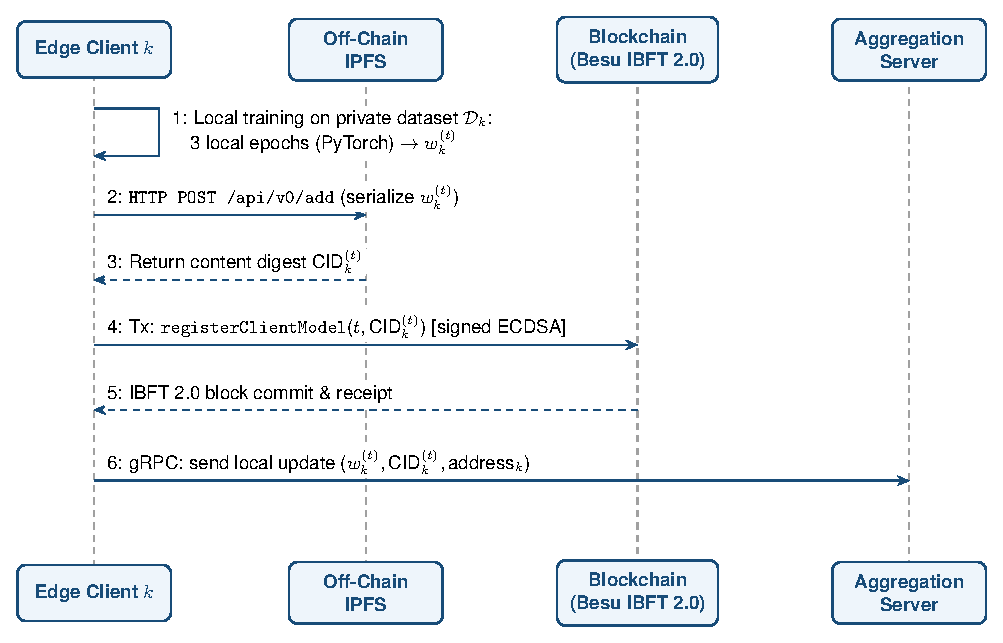
\includegraphics[width=\columnwidth]{figures/flujo_fase2_entrenamiento_registro.pdf}
    \caption{Phase 2: Local training at the client, parameter upload to IPFS, and signed transaction commitment to Hyperledger Besu.}
    \label{fig:flujo_cliente_entreno}
\end{figure}

\subsubsection{Phase 3: Upward Verification and Global Aggregation}
Upon receiving client updates at the aggregation coordinator (Figure~\ref{fig:flujo_servidor_agregacion}):
\begin{enumerate}
    \item For each client $k$, the server receives parameter payload $w_k^{(t)}$, identifier $\text{CID}_{k,\text{gRPC}}^{(t)}$, and client address $\text{address}_k$.
    \item \textbf{In-memory integrity verification:} The server deterministically computes the cryptographic digest of the received weight vector: $\text{CID}_{k,\text{calc}}^{(t)} = \text{Hash}(w_k^{(t)})$.
    \item \textbf{On-chain verification and double cross-check:} The server queries \texttt{getClientModel($t$, address$_k$)} from \texttt{FLRegistry}, retrieving $\text{CID}_{k,\text{onchain}}^{(t)}$, and enforces strict double equality:
    \begin{equation}
    \text{CID}_{k,\text{calc}}^{(t)} == \text{CID}_{k,\text{gRPC}}^{(t)} == \text{CID}_{k,\text{onchain}}^{(t)}
    \end{equation}
    This dual check counters two complementary threat vectors: if a malicious client commits a valid CID on Besu but transmits tampered weights over gRPC, or if a network adversary alters parameters in transit, $\text{CID}_{k,\text{calc}}^{(t)} \neq \text{CID}_{k,\text{onchain}}^{(t)}$; similarly, if the gRPC-reported CID does not match the signed transaction on Besu, verification fails immediately. In either case, the contribution is discarded prior to aggregation.
    \item The server executes FedAvg aggregation exclusively over verified contributions:
    \begin{equation}
    w^{(t+1)} = \sum_{k \in \mathcal{K}_{valid}} \frac{n_k}{n_{valid}} \, w_k^{(t)}
    \end{equation}
    where $n_k$ is the local sample count of client $k$ and $n_{valid} = \sum_{k \in \mathcal{K}_{valid}} n_k$.
    \item The server uploads the aggregated model to IPFS, obtaining $\text{CID}_{global}^{(t+1)}$, and anchors it on Besu by executing \texttt{updateModel(}$t+1$, $\text{CID}_{global}^{(t+1)}$\texttt{)}. Because \texttt{updateModel} is restricted by \texttt{onlyServer}, no outside party can overwrite the consolidated global model.
\end{enumerate}

\begin{figure}[htbp]
    \centering
    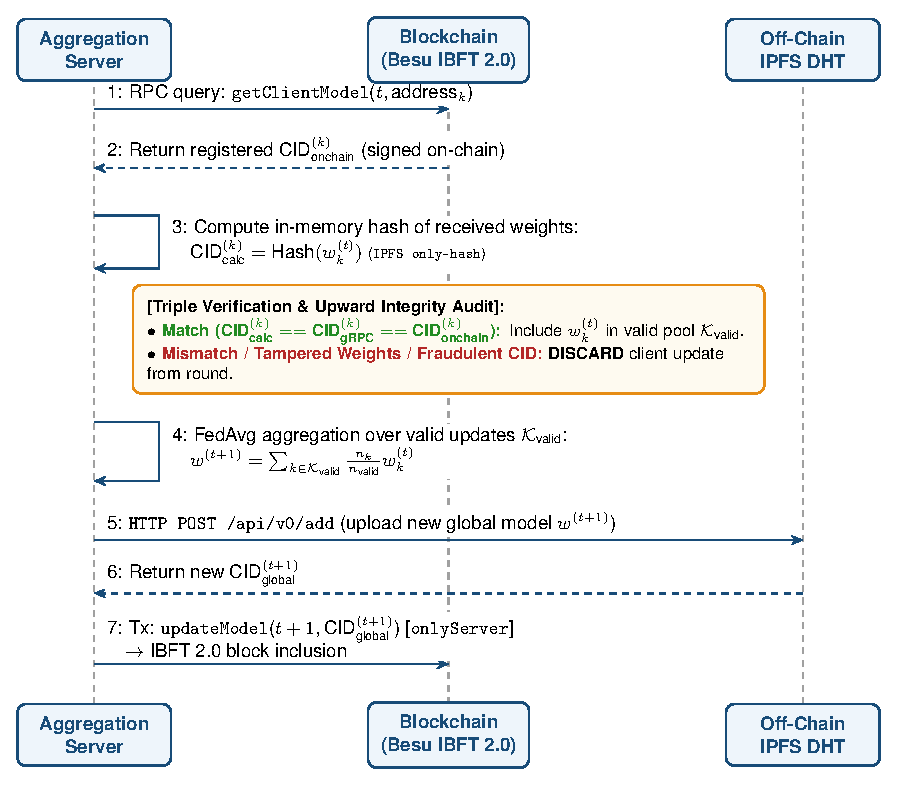
\includegraphics[width=\columnwidth]{figures/flujo_fase3_verificacion_agregacion.pdf}
    \caption{Phase 3: Upward verification at the aggregation coordinator: tensor integrity validation, on-chain cross-check, FedAvg aggregation, and global round commitment.}
    \label{fig:flujo_servidor_agregacion}
\end{figure}

\subsection{Ex-Post Auditing and Verifiability of FedAvg}
\label{subsec:auditoria_fedavg}
A distinctive architectural capability enabled by our hybrid decoupling is the ability to deterministically verify coordinator honesty retrospectively (\textit{ex-post}). In conventional federated setups, the aggregation server operates as a trusted black box: participants must trust that aggregated weights $w^{(t+1)}$ faithfully represent a weighted average over received contributions, without arbitrary omissions, unauthorized weight injections, or stealthy backdoors.

In our decoupled architecture, every round $t$ produces an immutable and reproducible audit trail linking the blockchain ledger to the content repository:
\begin{enumerate}
    \item \textbf{Participant identification $\mathcal{K}_t$:} Because Solidity \texttt{mapping} structures are non-iterable by EVM design, active participants in round $t$ are discovered deterministically by querying \texttt{ModelUpdated(round, modelHash, author)} event logs emitted during \texttt{registerClientModel} calls via standard RPC methods (\texttt{eth\_getLogs}), or from the permissioned consortium whitelist.
    \item \textbf{Local weight commitments:} Each participating client $k \in \mathcal{K}_t$ signs and registers its $\text{CID}_k^{(t)}$ in \texttt{clientHistory}, accessible via \texttt{getClientModel($t$, address$_k$)}.
    \item \textbf{Sample weighting factors $n_k$:} In balanced, homogeneous deployments (such as the evaluated experimental benchmark, where clients operate over equivalent IID partitions, $n_k = N / |\mathcal{K}_t|$), weighting factors are symmetric ($n_k / \sum n_j = 1/|\mathcal{K}_t|$). In heterogeneous settings (non-IID), scalar values $n_k$ can be embedded within the IPFS metadata descriptor or included as an event parameter, allowing exact reconstruction without exposing raw training samples.
    \item \textbf{Global model commitment:} The coordinator seals $\text{CID}_{\text{global}}^{(t+1)}$ in \texttt{history}, accessible via \texttt{getLastModel()} or direct round indexing.
\end{enumerate}

From this immutable audit trail, any consortium member or independent third-party auditor can execute a deterministic aggregation check without accessing private datasets:
\begin{enumerate}
    \item \textbf{Artifact retrieval:} The auditor queries Besu to retrieve active clients $\mathcal{K}_t$ and their committed $\text{CID}_k^{(t)}$, then downloads the binary parameter tensors $w_k^{(t)}$ from IPFS.
    \item \textbf{Input integrity validation:} It verifies that for each client $k \in \mathcal{K}_t$, the cryptographic digest of the downloaded weights strictly matches the on-chain committed $\text{CID}_k^{(t)}$.
    \item \textbf{Mathematical aggregation reconstruction:} It computes the canonical FedAvg aggregation:
    \begin{equation}
    \hat{w}^{(t+1)} = \sum_{k \in \mathcal{K}_t} \frac{n_k}{\sum_{j \in \mathcal{K}_t} n_j} \, w_k^{(t)}
    \end{equation}
    \item \textbf{Global model cross-check:} It serializes $\hat{w}^{(t+1)}$ and computes its content identifier $\text{CID}_{audit}^{(t+1)} = \text{Hash}(\hat{w}^{(t+1)})$. Finally, it evaluates whether $\text{CID}_{audit}^{(t+1)} == \text{CID}_{global}^{(t+1)}$, registered in \texttt{FLRegistry}.
\end{enumerate}
If $\text{CID}_{audit}^{(t+1)} \neq \text{CID}_{global}^{(t+1)}$, any coordinator deviation—whether due to biased weighting, participant omission, or unauthorized parameter tampering—is cryptographically, publicly, and non-repudiably proven. This verifiability transforms the centralized aggregator into a strictly accountable, provably honest orchestrator.

\subsection{Threat Model and Security Scope}
\label{subsec:modelo_amenazas}
To clearly delineate the defensive guarantees provided by the framework, this section defines the threat model, distinguishing between vulnerabilities mitigated by design and those that lie outside our scope.

\subsubsection{Mitigated Threats (In-Scope)}
\begin{itemize}
    \item \textbf{Man-in-the-Middle tampering}: A network adversary intercepting the gRPC channel who attempts to alter local parameter tensors sent to the server or global models delivered to clients. Discrepancies are intercepted immediately through element-wise numerical checks and on-chain CID verification.
    \item \textbf{Server equivocation / split-view attacks}: An untrusted or compromised coordinator attempting to deceive specific edge nodes by distributing divergent or altered global models (e.g., to facilitate active gradient inversion or localized performance degradation, as formalized by Carletti et al.~\cite{carletti2026detectability}). Because clients accept only weights whose content identifier strictly matches the authoritative commitment in \texttt{FLRegistry}, divergent distribution attempts are blocked locally.
    \item \textbf{Unauthorized global model injection}: Attempts by rogue participants or external adversaries to commit unauthorized global models to the blockchain are rejected by the EVM through the \texttt{onlyServer} modifier.
    \item \textbf{Contribution repudiation}: Elliptic curve digital signatures (ECDSA secp256k1) underpinning Hyperledger Besu transactions prevent participants from repudiating submitted parameter updates.
\end{itemize}

\subsubsection{Out-of-Scope Threats and System Boundaries}
\begin{itemize}
    \item \textbf{Semantic data and model poisoning with valid signatures}: If an adversary trains on poisoned datasets (e.g., label flipping or stealthy backdoors) but legitimately signs and registers the resulting model updates on Besu, cryptographic verification confirms provenance and integrity but cannot assess gradient statistical quality. Defense against semantic attacks requires pairing on-chain traceability with robust Byzantine aggregation rules (e.g., Krum~\cite{blanchard2017byzantine}, Median, Trimmed Mean) or forensic ex-post auditing of flagged contributions.
    \item \textbf{Private key compromise}: Cryptographic guarantees assume secure client key management. In industrial deployments, private keys must be secured via Hardware Security Modules (HSMs) or Trusted Execution Environments (TEEs).
    \item \textbf{Inference and gradient inversion attacks}: While our framework ensures integrity and provenance, it does not incorporate Differential Privacy (DP) or Secure Multiparty Computation (SMPC) to obfuscate shared gradients against reconstruction attacks~\cite{carletti2026detectability}.
\end{itemize}

\subsubsection{Privacy and Weight Exposure on IPFS}
On a public IPFS instance, any node knowing a model CID could retrieve parameter tensors and potentially attempt training data extraction. To protect model privacy in consortium deployments with stringent confidentiality requirements (e.g., autonomous fleets or healthcare), the framework supports two hardening mechanisms:
\begin{enumerate}
    \item \textbf{Private IPFS Swarm}: Configuring the IPFS daemon in private swarm mode using a shared key (\texttt{swarm.key}) and setting \texttt{LIBP2P\_FORCE\_PNET=1}. This prevents unauthorized nodes from connecting to the P2P overlay or fetching storage blocks.
    \item \textbf{Payload encryption at rest}: Encrypting serialized parameter vectors (e.g., using AES-256-GCM) prior to IPFS publication. Symmetric decryption keys can be distributed via asymmetric public-key cryptography to authorized consortium members or managed through Attribute-Based Encryption (ABE).
\end{enumerate}
